\section{Initialization and Optimization}
\label{sec:imp}
Based on our formulation described in Sec.~\ref{sec:method}, our method for joint registration and co-segmentation can be summarized in Algorithm \ref{alg:jrcs}.
%
In this section, we will explain in detail the parameter initialization and the user-guided optimization of our algorithm.

\begin{algorithm}[htb]
	\caption{Joint Registration and Co-segmentation (JRCS)}
	\label{alg:jrcs}
	\textbf{Input:}~~\\  
	$\{\vb{V}_m\}$: $M$ 3D point sets\\
	$\Theta^0$: Initial parameters\\
	$\{\beta_{ik}\}_{m}$: Layout prior\\
	\textbf{Output:}~~\\
	$\Theta^q$: Final parameters~~
	\begin{enumerate}
		\item $q\leftarrow1$
		\item \textbf{repeat}
		\item E-step: Use $\Theta^{q-1}$ to estimate $\alpha_{mik}^q$ according to Eq.~(\ref{equ:estep}) (use Eq.~(\ref{equ:bestep}) for the bilateral formulation);
		\item \textbf{if} $q < q_{alt}$  \textbf{then} Alter $\alpha_{mik}^q$ with $\{\beta_{ik}\}_{m}$ according to Eq.~(\ref{equ:alteralpha});
		\item M-step-a: use $\alpha^q_{mik}$, $\mathbf x^{q-1}_k$ to estimate $\{\mathbf{R}_{mn}^q\}$ and $\{\mathbf t_{mn}^q\}$ according to Eqs.~(\ref{equ:updateR})(\ref{equ:updatet});
		\item M-step-b: use $\alpha^q_{mik}$, $\{\mathbf{R}_{mn}^q\}$ and $\{\mathbf{t}_{mn}^q\}$ to update other parameters for Gaussian models according to Eqs.~(\ref{equ:updatexk})(\ref{equ:updatesigma})(\ref{equ:updatepk})(\ref{equ:updatey})  (or Eqs.~(\ref{equ:updatefk})(\ref{equ:updatefsigma}) for the bilateral formulation);
		\item $q \leftarrow q+1$
		\item \textbf{until} $q > q_{max}$
		\item \textbf{return} $\Theta^q$
	\end{enumerate}
\end{algorithm}



\subsection{Initialization}
\label{sec:imp:interact}
%
In our formulation, there are a large number of parameters that can not be easily initialized.
%
We provide an interactive tool to help with the initialization, as shown in Figure~\ref{fig:interact}. 
A set of boxes can be manually placed to indicate a rough segmentation of different objects in one point set. 
\mdf{Each object can be roughly indicated by multiple boxes.} 
%User can use boxes with different colors to indicate a scene layout for different objects in one of the point sets.
%
Based on the roughly placed boxes, we can initialize the parameters in our formulation. 

\noindent\textbf{Number of objects $N$}: $N$ is naturally determined as the number of placed box groups in the point set.

\noindent\textbf{Number of Gaussian models in each object $\{K_n\}^N_{n=1}$}: While objects in an indoor scene have varying volumes, we use different number of Gaussian models for objects according to their volumes. We set $K_n$ as 
\begin{equation}
\label{equ:K_n}
K_n=\frac{V_n}{\sum V_n}K_{all},
\end{equation}
%
where $V_n$ represents the total volume of the boxes for $O_n$. 
The total number of Gaussian models $K_{all}$ in the scene is initialized as $\frac{1}{2}\big(median(\{L_m\}^M_{m=1}\big)$, where $L_m$ is the number of points in $\vb{V}_m$. 
This is an empirical choice borrowed from \cite{Evangelidis2014}.

\begin{figure}
	\centering
	\includegraphics[width=.45\linewidth]{images/interact01.png}
	\includegraphics[width=.45\linewidth]{images/interact02.png}
	\includegraphics[width=.45\linewidth]{images/interact03.png}
	%\includegraphics[width=.3\linewidth]{images/interact04.png}
	%\includegraphics[width=.3\linewidth]{images/interact05.png}
	\includegraphics[width=.45\linewidth]{images/interact06.png}
	\caption{\label{fig:interact}
		From the $1^{st}$ to the $4^{th}$, the four images show the procedure of interaction:
		Given all the point sets as input, the user picks one point set and place boxes to indicate the layout for this point set. The box in white is the box currently under editing. The boxes in other colors are boxes placed to represent object layouts. One color represents one object. The interaction allows multiple boxes to represent same object. (e.g. the desk is represented by three boxes in same color)}
\end{figure}

\noindent\textbf{Gaussian parameters $\{p_k,\mathbf{x}_k,\Sigma_k\}_{k=1}^{K_{all}}$}:
We initially set $p_k=\frac{1}{K_{all}}$, which means each Gaussian model is equally weighted at the beginning. 
%
%For the Gaussian centroids $\{\mathbf{x}_k\}$, we first allocate memory for total $K_{all}$ Gaussian centroids and then separate them into $N$ groups to represent $N$ objects. 
%Each group has $K_n$ Gaussian centroids based on Eq.~(\ref{equ:K_n}). We implement this by recording the start and end indices of the $N$ objects. In other words, we record $\{0,K_1,K_1+1,K_1+K_2,...,K_S+1,K_S+K_n,...\}$. 
For object $O_n$, we initialize its $K_n$ Gaussian centroids $\{\mathbf{x}_k\}_{K_S+1}^{K_S+K_n}$ as random positions uniformly distributed on the surface of a sphere, whose radius $r$ is chosen as the median of the radius of the input point sets.
%
%
The radius of a point set is defined as half of the length of diagonal line of its axis-aligned bounding box.
 
%
The center of the $n^{th}$ sphere is $\mathbf{c}_n=(0,0,z_n)$, where $z_n\in \{-(N-1)r,-(N-3)r,...,(N-1)r\}$.
%
This means that the object models are vertically arranged in latent space as shown in Figure~\ref{fig:teaser}(c). 
%
We choose vertical arrangement for groups of object merely for the convenience of visualization.
%
Figure~\ref{fig:iter}(b)\cxj{"E00"} shows an example of the initial Gaussian centroids of a scene with three objects.
%
The variance $\{\Sigma_k\}$ are all initialized as $\Sigma_k=\sigma^2 \vb{I}$ in which $\sigma=r$.
%
Without any prior knowledge, such initialization for Gaussian parameters put all the objects at similar starting points and they can compete fairly to group points in the input point sets. If we set $r$ differently for each object based on the size of input boxes, it could be easily stuck to a local minimum that all the points are assigned to the largest object.

\noindent\textbf{Transformations} $\{\phi_{mn}\}_{m=1,n=1}^{M,N}=\{\mathbf{R}_{mn},\mathbf{t}_{mn}\}_{m=1,n=1}^{M,N}$:
Since we have chosen spheres as the initial shapes, we can initialize all the $\mathbf{R}_{mn}$ to an identity matrix.
%
%For sphere, the different initial orientation makes little differences.
%
For translations, we initialize them as $\mathbf{t}_{mn}=- \mathbf{c}_n$ so that all the object models start with position at the origin point when they are transformed to the space of each input set. 
%
However, if boxes are manually placed in the point set $\vb{V}_m$, we treat the associated $\mathbf{t}_{mn}$ differently:
%
\begin{equation}
	\label{equ:initt}
	\vb{t}_{mn}=\frac{\sum_{\vb{v}_{mi} \in B_n}\vb{v}_{mi}}{N(B_n)}-\vb{c}_n, 
\end{equation}
where $N(B_n)$ here is the number of points enclosed by the manually placed boxes indicating object $O_n$.


\begin{figure}
	\centering
	\includegraphics[width=\linewidth]{images/localoptimal/localoptimal}
	\caption{\label{fig:localoptimal} An example result when our algorithm converges to a local optimal. (a) The segmentation result in six point sets of this local optimal. (b) The Gaussian centroids of the latent object models. It shows that the chair and the table are not perfectly segmented. \cxj{change colors of the chair and the table.}}
\end{figure}

\subsection{Layout Constrained Optimization}
\label{subsec:optimzation}

Our formulation inherits the disadvantage of easily getting stuck to a local optimal from the EM framework.
%The expectation maximization framework is easily converged to a local optimal. 
From a random initialization for object models,
\cxj{not randomly initialized, its on a sphere surface}, the EM framework sometimes fails to get a globally optimal solution, as Figure~\ref{fig:localoptimal} shows. 
The chair and the table are not perfectly segmented, \cxj{starting from the initial sphere-shape object models.} 
%
To cope with this problem, we adopt the user placed boxes as soft constraints to guide the optimization and confine the shape of generated object models. 
Such constraints are enforced by altering the posterior probability as
\begin{equation}
	\label{equ:alteralpha}
	\alpha_{mik}^*=\frac{\alpha_{mik}\beta_{mik}}{\sum_{i,k}\alpha_{mik}\beta_{mik}}
\end{equation}
%
where $\beta_{mik}$ is the prior probability according to the boxes, defined as:
\begin{equation}
	\beta_{mik}=\left\{
	\begin{array}{lcl}
		1,& &\mathbf v_{mi} \in B_n\\
		\exp(-\frac{\min_{\mathbf v_{mj}}|| \mathbf v_{mi} - \mathbf v_{mj} ||_2^2  )}{
			2r^2}),& &\mathbf v_{mi} \notin B_n~and~\mathbf v_{mj} \in B_n\\
	\end{array} \right.
\end{equation}
%
where $B_n$ is a set of points that are enclosed by the boxes used to represent object $O_{n}$. 
%
%The $k^{th}$ Gaussian model is predefined to be one of the Gaussians used to represent $n^{th}$ object.
$\min_{\vb{v}_{mj}}|| \vb{v}_{mi} - \vb{v}_{mj} ||_2^2$ is the minimum distance from a point $\vb{v}_{mi}$ to the points $\{\vb{v}_{mj}\}$ in object $O_n$.
%the squared Euclidean distance from point $v_{mi}$ to the point set $B_n$, as we define the distance from a point to a point set as the minimum distance from the point to any point inside the point set. 
%$L$ here is a constant with $R=2r^2$, and 
$r$ is the median of the radius of input point sets.
%   
%The radius of a point set is half of length of diagonal line of its axis-aligned bounding box.
This alteration on posterior probability is only done for the points in the point set where boxes are manually placed. 
%

\begin{figure*}
	\centering
	\includegraphics[width=\linewidth]{images/Initialization/iters_merge}
	\caption{\label{fig:iter} This figure shows an example of our algorithm converging with increasing number of iterations.
		(a) shows the curve of objective function - iteration number. The objective value is calculated according to (\ref{equ:obj3}). Note that the curve is not monotonic increasing, which makes it difficult to set a stop condition based on our objective.(b) shows three input point set as examples out of 12. Column "00" shows the input point sets and the initial Gaussian centroids, among which "B00" has two images the left one  is the input layout (boxes) which is only placed in the first point set. The column "01"-"08" shows result of segmentation (in row "B"-"D") and Gaussian centroids (in row "E") at different iteration numbers $q$. The $q$ is shown at top of each column. The row "A" shows highligted areas of "B01"-"B08" }
\end{figure*}

This alteration can prevent the object models from deforming into an arbitrary shape.
%
%In Figure~\ref{fig:localoptimal}, the $2nd$ and $3rd$ object has deformed into a combination of two objects due to lack of constraint.
%
Figure~\ref{fig:iter} demonstrates the converging procedure with box constraints. 
%
We can see that with the boxes placed in one point set as constraints, our framework converges to a good segmenation result. The point sets are finally segmented to three objects, and the object models develop from a initial sphere shape at $q=1$ to a dense point cloud which fits the input point sets well. 
%
However, in Figure~\ref{fig:iter}(a), the objective function is not monotonically increasing. 
This is due to our alteration on the posterior probability in Eq.~(\ref{equ:alteralpha}). This alteration is a quite brutal solution to enforce the shape constraint and it will interfere with the convergence of EM algorithms.
% 
This makes it difficult to set a stop criteria based on the objective value. 
We now stop the iteration when the maximum iteration number $q_{max}$ is reached.
% as shown in Algorithm~\ref{alg:jrcs} step 8.
 
As highlighted in Figure~\ref{fig:iter}(b)"A01"-"A08", the segmentation in the first point set seldom changes until the last few iterations. 
%
This is due to the alteration in Eq. (\ref{equ:alteralpha}) as well. 
%
In order to constrain the object shape, we do alteration on the posterior probability of the point set where boxes are placed. This alteration is only done in $q_{alt}$ iterations as shown in Algorithm~\ref{alg:jrcs} step 4. 
However, the initial segmentation based on the boxes is not accurate. 
Therefore, we no longer do such alteration in the last few iterations and let the algorithm to refine the segmentation based on the result of registration. 
We set $q_{alt}=q_{max}-10$ for all experiments in this paper.

For initialization and object shape constraint, the boxes are first roughly placed in one point set only. 
%When the proposed algorithm 
\mdf{In more challenging cases, if the user is not satisfied with the segmentation and registration results, we also allows the user to add more box-shape constraints in different point sets to refine the results.}
%For such cases, our implementation allows placing more constraints in other point sets (even during the optimization process). 
The same alteration as Eq. (\ref{equ:alteralpha}) is performed in optimization. We will discuss an example of such case later in Sec~\ref{subsec:interact}.